\chapter{Early experiments}

\epigraph{And you may ask yourself \\ "Well\dots how did I get here?"}{Once in a Lifetime \\ Talking Heads, 1981}

In this chapter I showcase my journey, experience, pitfalls, breakthroughs and what led me to working on this  thesis, and I will try to be open, detailed, celebratory, and critical.

\section{Microcontrollers for arts}

I learned how to program microcontrollers around 2010 as an undergraduate student of electrical engineering in Chile, with PIC microcontrollers, C\# and Windows machines. In parallel, with some classmates we discovered the Arduino microcontrollers, and with my friend Braulio we built a robotic guitar tuner, where the Arduino detected the pitch of a string, and made a motor move the tuning gear of the string to match the desired pitch.

Fast forward to thesis in 2013, we had to complete a capstone project and implement many low-level programming techniques, so Arduinos were not allowed because they were considered a shortcut. With my friend Guillermo we built a robotic device with a PIC microcontroller programmed with C\#. Our code was very specific to that particular chip and project, and hardly reusable or interesting for a wider audience, in a stark contrast to my experience using Arduino, where projects could be shared and remixed. I never programmed PICs again, and Arduinos became a huge part of my practice. I am grateful about the community's efforts on sharing resources online, and the extensive documentation available.

After graduation I freelanced as a software and technology designer and developer for artists. I learned computer protocols and networks, and wrote custom software for live multimedia performance, theater and music, and software deployed on iPads and cellphones. I discovered Processing, a project that Arduino was based on, and continued learning code on my own. With Processing I was able to learn how to build apps with computer graphics, interactivity, and it quickly became central to my practice and work.

\begin{figure}[ht]
  \centering
  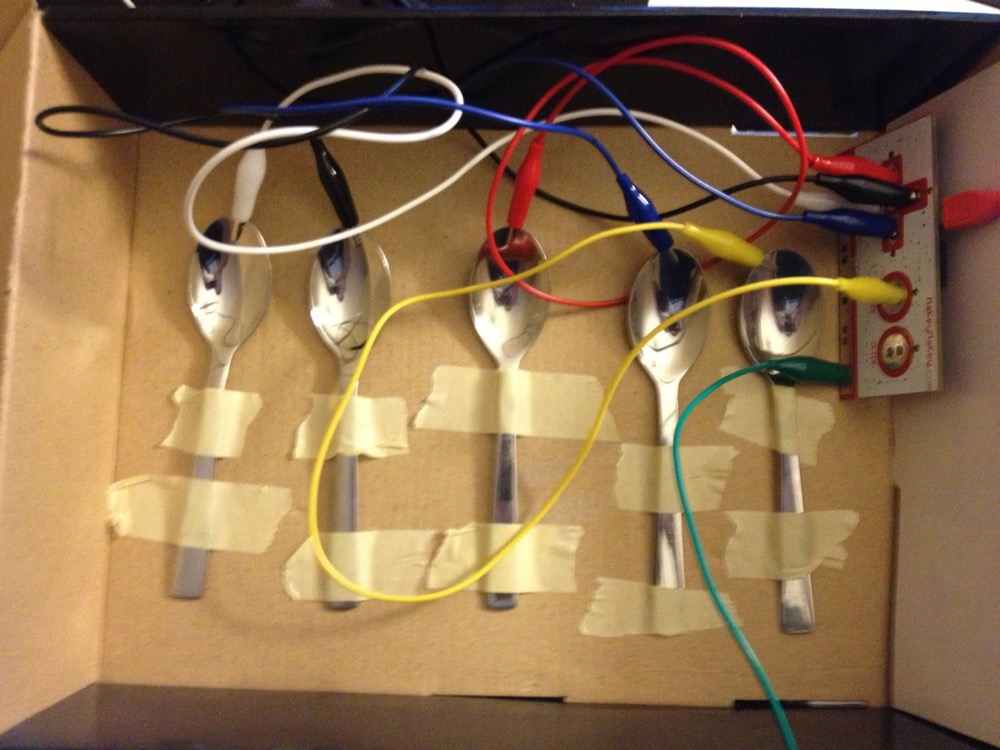
\includegraphics[width=0.75\linewidth,height=0.25\textheight,keepaspectratio]{images/makey-makey-spoons.jpg}
  \caption{Spoon synthesizer made with Makey Makey}
  \caption*{Picture taken by myself}
  \label{fig:makey-makey-spoons}
\end{figure}

Realizing that I needed a bigger community of people to learn media arts from, I researched communities where I thought I could learn this craft in an focused and immersive way, so I applied to New York University's Interactive Telecommunications Program, where I joined as a graduate student in 2015.

In my first semester I took the amazing class Introduction to Physical Computing, with one of Arduino's co-creators Tom Igoe, and I learned about haptic design, open source hardware and software, and physical computing education.

I was introduced to a wider ecosystem of microcontrollers beyond Arduino, like the Teensy by PJRC, which captivated me by its USB MIDI capabilities, which allowed for standalone MIDI operation, and the creation of plug and play devices that needed no additional setup or scripting. Also by its audio library, which allowed me to create interactive standalone experiences, playing audio samples and applying audio effects.

At NYU ITP I slowly learned about hardware,  but mostly about web and scripting, and my thesis concentrated on open source, performance art, with only a small hardware component in the form of a Raspberry Pi computer with a countdown timer to my projected death time, according to data by the United Nations, based on my assigned-at-birth-gender and my birth place.

After graduating from NYU ITP I focused on media arts education, writing tutorials, teaching introduction to programming workshops for artists.

When I joined MIT Media Lab in 2019, I made the conscious decision of focusing on hardware, to give my creations a life outside of my computer, also inspired by newer restrictive developments by Apple, such as restricting the use of apps created by unregistered developers. In my first semester, which ended up being the only on-campus semester I had, I was introduced by my friend Will Freudenheim to the Shbobo synthesizers by Peter Blasser.

I was partially aware of the instruments made by Peter Blasser, in particular the analog ones.

While at MIT Media Lab, I was delighted by the newer versions of Teensy, which are even faster and more powerful, and which led me to start designing handheld samplers for field recordings, and other standalone devices.

This in turn led me to review the current NYU ITP materials for physical computing, where they currently stopped using the now classic Arduino Uno, and have incorporated in their teaching the new series of Arduino Nano microcontrollers, which I based my thesis on.

In particular, the Arduino Nano 33 BLE Sense I am using, comes with 9 sensors, to measure and detect acceleration, movement, distance, color, and a microphone. This is an amazing breakthrough, since now we can use all this data without having to purchase, install, or calibrate the sensors.

I am using the Arduino's sensors to gather multimedia input data, analyze it with machine learning, and then responding with multimedia outputs.

\section{Machine learning}

My first experiment with creative machine learning, was with my NYU ITP classmate Corbin Ordel, who was a student at Gene Kogan's machine learning class, and we teamed up to hack a project we called Piano Die Hard, built with open source tools such as Wekinator, Arduino, openFrameworks, and using the machine learning algorithm KNN. We created a video database of explosions in the Die Hard movie franchise, and another one of other 1980's movies with no explosions, and we trained our machine learning algorithm to distinguish between the categories explosion and no explosion. We featured this project at a NYU ITP show, were written up at the Daily Beast newspaper, and exhibited our work at the alt-ai conference.

In 2017, while I was finishing my appointment as research resident at NYU ITP, Cristóbal Valenzuela had started the project RunwayML as his master's thesis, which is now a company led by Cristóbal, Alejandro Matamala and Anastasis Germanidis.

At NYU ITP I also saw the first experiments with deeplearn.js, later TensorFlow.js, which soon became the foundation of the ml5.js library, a wrapper for TensorFlow.js, for on-the-browser machine learning.

I decided I wanted to dip my toes in machine learning, so I took a month-long intensive class at the School of Machines in Berlin, Germany, facilitated by Gene Kogan and Andreas Refsgaard, and organized by Rachel Uwa.

A big inspiration for this thesis has been the book on GANs by Casey Reas, published by Anteism, as of 2021 on its second edition. It’s an arts-first book that contextualizes the use of machine learning algorithms for the creation of images, and uses the metaphor of these algorithms as being similar to the development of the camera. Artists don’t need to understand all the physics or mechanics behind a camera in order to make art with it, but it can help to understand it too. I think machine learning is also a game changer for instrument making, and machine learning introduces new civic complexities, and my thesis tries to follow the example of this book, to introduce the technology and contextualize for a new generation of artists and instrument makers.

Since many machine learning projects rely on proprietary hardware, such as NVIDIA GPUs, or rely on the cloud for faster compilation times, for this thesis I decided to make open source machine learning projects that people could read and understand and remix and hack.

TODO: mention the impact of the documentary Coded Bias, and how these researchers impacted my desire to make my thesis. Also mention how right before pandemic I had started a pottery class, with the intention of making clay-based instruments for thesis, as a metaphor of making code and hardware and software feel fluid and not static, I want to empower people to program, in particular machine learning because of its dangerous implementations by oppressive governments and corporations, and in particular for arts, for making artists dream come true.

\section{Interfaces and instruments}

I am an enthusiast of new interfaces and instruments for music and media art production.

asdf
